\documentclass[12pt]{article}
\usepackage[paper=a4paper,left=20mm,right=20mm,top=30mm,bottom =30mm]{geometry}
\usepackage[utf8]{inputenc}
\usepackage[T1]{fontenc}
\usepackage{stmaryrd}
\usepackage{setspace}
\usepackage{mathrsfs}
\usepackage[ngerman]{babel}
\usepackage{amssymb}
\usepackage{amsmath}
\usepackage{fancyhdr}
\usepackage[dvips,unicode,colorlinks,linkcolor=black]{hyperref} 
\usepackage{graphicx}
\usepackage{float}

\pagestyle{fancy}
\lfoot{}
\rfoot{Paul Kremser, Tobias Grussenmeyer}
\cfoot{\thepage}
\fancyhead[L]{FPI Versuch: Hanle - Effekt}
\renewcommand{\headrulewidth}{0.6pt}
\renewcommand{\footrulewidth}{0.6pt}
\setlength{\headheight}{16pt}
\setlength{\parindent}{0pt}
% Für die Wahl der Schriftart
\newcommand{\changefont}[3]{
\fontfamily{#1} \fontseries{#2} \fontshape{#3} \selectfont}

\begin{document}
% keine Hurenkinder und Schusterjungen
\clubpenalty = 10000
\widowpenalty = 10000 
\displaywidowpenalty = 10000

\onehalfspacing
% Schriftart
\changefont{ptm}{m}{n} 

\begin{titlepage}
\author{Paul Kremser, Tobias Grussenmeyer}
\title{Versuch: Hanle - Effekt}
\date{Versuchsdurchführung: 9. und 12. Oktober 2009} 
\maketitle
\thispagestyle{empty}
\end{titlepage}


\tableofcontents
\thispagestyle{empty}
\newpage
\pagenumbering{arabic}
\section{Überblick}
Mit dem Versuch soll die Lebensdauer angeregter Zustände des Queckilberatoms bestimmt werden. Grob gesagt werden hierzu Quecksilberatome in einer 
Quarzzelle durch polarisiertes Licht angeregt. Durch ein von außen angelegtes Magnetfeld wird die Richtung
in der die angeregten Atome wieder abstrahlen beeinflusst.

\section{Aufgabestellung}
Bestimmung der Lebensdauer des angeregten $6s6p \quad ^3P_1$ Zustands des $Hg$-Atoms durch Messung des Hanle-Signals in Abhängigkeit vom Dampfdruck
des Quecksilbers für verschiedene Polarisationsrichtungen des einstrahlenden Lichts. Dokumentation der Änderung der effektiven Lebensdauer durch
\textit{Coherence Narrowing}

\section{Theoretische Grundlagen}

Wir nutzen den Hanle-Effekt zur bestimmung der Lebensdauer angeregter  Zustände im Hg-Atom. Dazu bestrahlen wir die Atome mit linear polarisiertem Licht dessen Wellenlänge dem Übergang des zu untersuchenden Zustands entspricht bestrahlt. Die bestrahlten Atome werden dadurch angeregt und strahlen ebenfalls Lichtdieser Wellenlänge und polarisation aus (Resonsnzfluoreszenz). Beobachtet man die Atome nun aus der zur polarisation parallelen Richtung so sieht man zunächst keine Strahlung. Legt man senkrecht zur Polarisationsrichtung ein äusseres Magnetfeld an so sieht man bei Variation dieses Feldes auch eine Variation der Intensität. Dies wird als Hanle Effekt bezeichnet.

\subsection{Klassische Deutung}
Bei klassischer Betrachtungsweise schwingt das angeregte Atom als Dipol entlang der Polarisationsachse. Es handelt sichalso um einen gedämpften Oszilator, das Atom schwingt bis es durch die Strahlungsdämpfung wieder zur Ruhe kommt. Betrachtet man nun diesen Dipol parallel zur Schwingunsachse so sieht man keine Strahlung da ein Dipol nie in dieser Richtung abstrahlt. Legt man nun senkrecht zur Schwingung ein Magnetfeld an so beginnt das elektron aufgrund der Lorentzkraft mit der Lamorfrequenz um die Feldrichtung zu präzedieren. Diese Frequenz berechnet sich zu:
\begin{align}
 \omega_L=\frac{g_j \mu_B H}{\hbar}
\end{align}
wobei $g_j$ der Landesche Faktor und $\mu_B$ das Bohrsche Magneton ist. In einer zur Feldachse senkrechten Ebene kommt es dadurch zu einer rosettenartigen Figur der Elektronenbahn.
\\
Die Intensitätsverteilung des Dipols ist im wesentlichen eine $sin^2(\vartheta)$ Verteilung ($\vartheta$ ist der
Winkel zwischen Dipolachse und Beobachtungsrichtung). Setzt man nun $\vartheta = \omega_L t$ und beschreibtdie Dämpfung mittels den Term $e^{-t/\tau}$, mit $\tau$ als mittlerer Lebensdauer des angeregten Zustands so folgt die Strahlungsintensität zu:
\begin{align}
 I = C \int \limits_{0} \limits^{\infty} e^{-\frac{t}{\tau}}sin^2(\omega_L t) dt
\end{align}

Dieses Integral ergibt augewerteteine inverse Lorentzkurve, $C$ ist eine Proportionalitätskonstante. Ist die Polarisationsrichtung um $\pi/2$ zur Beobachtungsrichtung gedreht so ergibt sich eine normal Lorentzkurve. In beiden Fällen gilt für die Halbwertsbreite $\omega_{\frac{1}{2}}$:
\begin{align}
 \omega_{\frac{1}{2}}= \frac{\hbar}{g_j \mu_B\tau}
\end{align}

Daraus folgt dann für die Lebensdauer, wenn $H_{\frac{1}{2}}$ die Feldstärke bei halber Höhe der vollen Intensität ist:
\begin{align}
 \label{livetime_classic} \tau = \frac{\hbar}{2 g_j \mu_B H_{\frac{1}{2}}}
\end{align}

\subsection{Quantenmechanische Deutung}
Der Hanle Effekt ist ein spezialfall des sogenanten \textit{level-crossing}. Unter level-crossing versteht man folgendes:

Liegt eine Feinstrukturaufspaltung in verschiedene Zeeman-Niveaus bereits ohne äußeres Magnetfeld vor, so können die verschiedenen Niveaus durch Anlegen eines Feldes zur Überkreuzung gebracht werden, d. h. bei einer bestimmten Feldstärke können zwei Niveaus energetisch zusammenfallen. In diesem Bereich findet man eine merkliche Änderung der Intensität der Fluoreszenzstrahlung.

Der Hanle Effekt tritt beiFeldstärke null auf, dh die Energien der Feinstrukturauflösung fallen bei Feldstärke Null zusammen. Der Intensitätsverlauf kann quantenmechanisch hergeleitet werden, dazu kann man bei diesem Versuch die Breit-Formel verwenden, eine Ratengleichung, welche die Absorption und Reemission von Photonen (mit der Polarisation von $f$ bzw. $g$) in der Resonanzzelle beschreibt. Für ein System mit Grundzustand a und zwei sich kreuzenden Zuständen b und c lässt sich die Rate aufspalten, mit $\nu(b,c)$ als Frequenzdifferenz der angeregten Zustände.
\begin{align}
 R(f,g)=c\left[ R_0+\frac{A}{1-2\pi i \tau \nu (b,c)}+\frac{A^*}{1-2\pi i \tau \nu (b,c)}\right]
\end{align}

Man erhält für ein imaginäres A einen Intensitätsverlauf in Form einer Dispersionskurve und für ein reelles A eine Lorentzkurve. Von den drei Komponenten in die sich ein $3_P^1$-Term aufspaltet, nämlich $m = 0$ und $m = \pm 1$, beobachten wir nur die Strahlung der $m = \pm1$-Komponenten. A ist in diesem Fall reell und die Energieaufspaltung im Magnetfeld beträgt:
\begin{align}
 \Delta \nu = \frac{2 g_j \mu_B H}{h}
\end{align}

Für die Halbwertsbreite der Lorentzkurve erhält man:
\begin{align}
 \Delta \nu_{\frac{1}{2}} = \frac{1}{\pi \tau} = \frac{2 g_j \mu_B 2 H_{\frac{1}{2}}}{h}
\end{align}

und somit erhält man für die mittlere Lebensdauer wieder:
\begin{align}
 \label{livetime_quantum} \tau = \frac{h}{4 g_j \mu_B \pi H_{\frac{1}{2}}} = \frac{\hbar}{2 g_j \mu_B H_{\frac{1}{2}}}
\end{align}

\subsection{Coherence Narrowing}
Hierbei handelt es sich um einen Effekt der die mittlere Lebensdauer länger erscheinen lässt. Dabei wird ein Atom in der Nähe des angeregten durch die Strahlung des ersteren selbst angeregt. Dieses Schwingt unter Beibehaltung der Präzession, Phase und Raumorientierung der Dipolschwingung des ersten Atoms. Dieser Prozess kann mehrfach auftreten, seine Wahrscheinlichkeit hängt vom Dampfdruck der beobachteten Substanz ab. Der Dampdruck steigt mit der Temperatur, wesshalb wir Messungen bei verschiedenen Temperatur durchführen um dann auf den Wert $T=0K$ zu extrapolieren.
\newpage

\section{Versuchsaufbau}
\begin{figure}[H]  
\centering
\includegraphics[width=0.7\linewidth]{pictures/Aufbau.ps}
\caption{Versuchsaufbau des Hanle-Effekts}
\end{figure}

Als Lichtquelle dient eine HF-induzierte Gasentladung in einer Quecksilberdampflampe. Das Lich gelangt über zwei Linsen, einem Interferenzfilter und einem Polarisator in die mit Quecksilberdampf gefüllte Resonanzzelle aus Quarz. Die erste Linse macht das Licht parallel, der Interferenzfilter filtert die zur Anregung des $3_P^1$-Zustands benötigte Spektrallinie, der Polarisator polarisiert das Licht in die gewünschte Richtung und die zweite Linse fokussiert das Licht in die Zelle. Die Zelle wird über ein Kühlsystem aus Peltierelement und Wasserkühlung gekühlt um die Messung bei verschiedenen Temperaturen (also verschiedenen Dampfdrücken) zu ermöglichen. Um die Zelle herum sind drei Helmholtzspulenpaare angebracht. Zwei davon sind zur Kompenstion der von externen (ua Erdamgnetfeld) Stöhrfeldern, das dritte ist zum erzeugen des für den Hanle Effekt nötigen Magnetfeldes, dieses wird wärend des Versuchs variiert. Senkrecht zur Einfallsrichtung des Lichts wird die erzeugte Resonanzstrahlung Über einen Lichtleiter zum Photomultiplier geführt. Von dort wird das Signal an ein Elektrometer weitergegeben, das über ein Osziloskop an einen Computer angeschlossen ist, mit dem das Signal dann aufgezeichnet wird.
\newpage

\section{Durchführung}
Zunächst Stellten wir die Kompensierenden Magnetfelder ein und justierten den Polarisator auf $90^\circ C$. Wir erhielten ein sauberes symetrisches Hanle Signal. Dann kühlten wir Die Resonanzzelle auf die minimal ereichbare Temperatur (zunächst $-11^\circ C$) und nahmen wärend des Aufwärmens Messungen bis $10^\circ C$ auf. Danach justierten wir den Polarisator auf $\pm 45^\circ C$ und nahmen je eine Dispersionskurve auf. Zuletzt kühlten wir wieder (über 3 Stunden, laut Anleitung wird nach einer Stunde die minmale Temperatur erreicht) um die $0^\circ C$-Polarisationrichtung zu vermessen. Leider erreichten wir hier nur noch eine Temperatur von $-5^\circ C$. 

\section{Auswertung}
Die genutzte Formel zum fitten der Lorentzkurve lautet:
\begin{align}
 y(x) &= y_0+\frac{2A}{\pi}\frac{\omega}{4(x-x_c)^2+\omega^2}+b_x \\
\notag \textnormal{ mit }~~~~ y_0 &\widehat{=} \textnormal{ Y-Achsenoffset } \\
\notag A &\widehat{=} \textnormal{ Fläche } \\
\notag x_0 &\widehat{=} \textnormal{ X-Koordinate des Peaks } \\
\notag \omega &\widehat{=} \textnormal{ Halbwertsbreite der Kurve } \\
\notag b &\widehat{=} \textnormal{ Steigung des linearen Terms zur berücksichtigung der Temperatur}
\end{align}

Bei den zum Fitten verwendeten Messpunkten beschränkten wir uns auf einen Bereich von $0,7A$ um den Peak der Kurve, um Unregelmässigkeiten am Rand der Messung auszufiltern. Der Parameter $\omega$ dieser Kurve liefert uns direkt die Halbwertsbreite in Ampère. Aus dieser können wir die Magnetfeldstärke $H_{\frac{1}{2}}$ in Tesla bei halber Intensität bestimmen:
\begin{align}
 2H_{\frac{1}{2}}= 3,363\cdot 10^{-4} \omega
\end{align}

Also folgt mit Gleichung \ref{livetime_classic} oder \ref{livetime_quantum} die Lebensdauer in Sekunden:
\begin{align}
 \tau = \frac{\hbar}{2g_j \mu_B H_{\frac{1}{2}}} = \frac{\hbar}{g_j \mu_B\cdot 3,363\cdot 10^{-4} \omega}
\end{align}

mit dem Fehler:
\begin{align}
 s_{\tau}=\tau \frac{s_{\omega}}{\omega}
\end{align}







\section{Zusammenfassung}

\end{document}
